Recently, it has been recognized that very strong electric and magnetic fields are created at early times of ultra-relativistic heavy-ion collisions. In Fig.~\ref{fig:EMfield}, the time dependence of the magnetic ($\rm B_{y}$) and electric ($\rm E_{x}$) fields in \PbPb collisions at $\sqrtsNN=$ 2.76$\UTeV$ with impact parameter b=9.5$\Ufm$ is presented for a system with electric
conductivity $\rm \sigma_{el}=$0.023$\Ufm^{-1}$. The space-time evolution is obtained as solution of the Maxwell's equations as developed in \cite{Gursoy:2014aka}. The magnetic field produced in non-central heavy ion collisions is dominated by the $\rm B_{y}$ component which induces a current in the $xz$ plane while the time dependence of $\rm B_{y}$ generates an electric field which is directed in the $x$ direction. The combined effect of both fields is a current in the $xz$ plane.
\begin{figure}
\centering
\resizebox{0.5\textwidth}{!}{  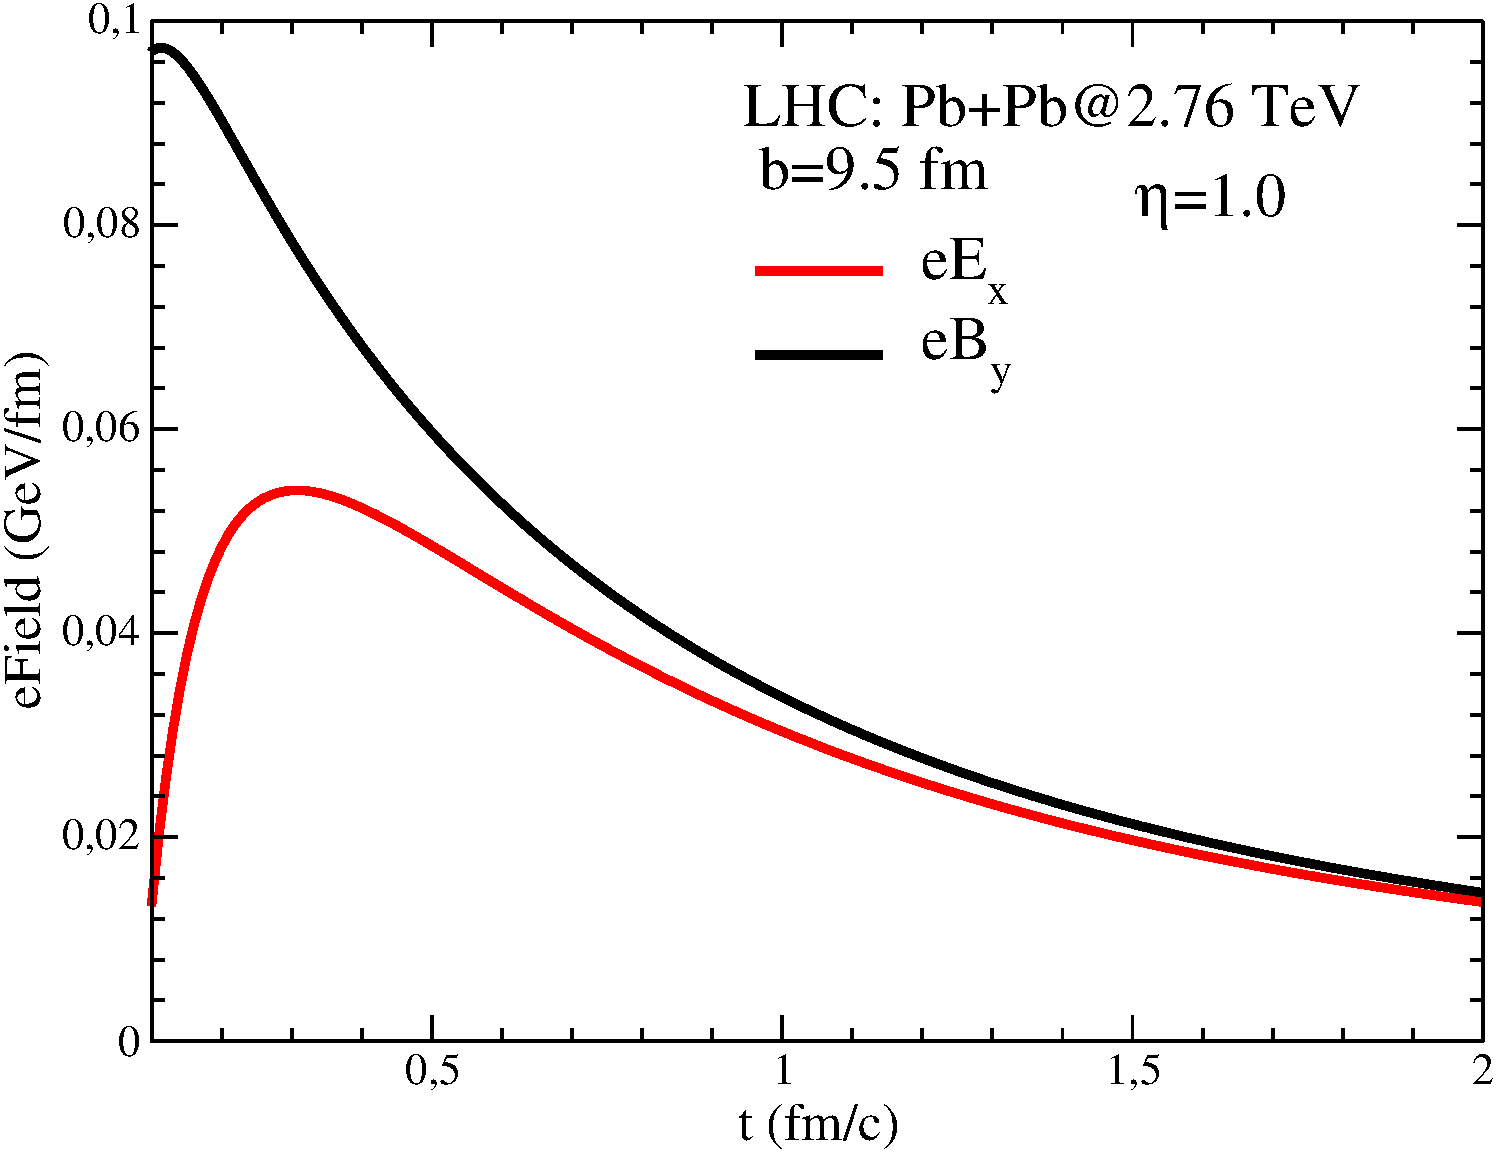
\includegraphics{hf/figures/EMfield_evolution.pdf}}
\caption{Time evolution in the forward rapidity region of the magnetic field $\rm B_{y}$ and electric field $\rm E_{x}$ in \PbPb collisions at $\sqrtsNN=$ 2.76$\UTeV$ with impact parameter b=9.5$\Ufm$.}
\label{fig:EMfield}
\end {figure}

The presence of early magnetic fields produced in heavy-ion collisions is expected to have an effect on the charm directed flow~\cite{Das:2016cwd,Chatterjee:2018lsx,Plumari,Sandeep}, resulting in a $\vone$ value larger than that of lighter particles (short charm formation time and therefore sensitive to the maximum magnetic field strength), and opposite for particles with charm and anti-charm (due to the Lorentz force). Also the initial vorticity of non-central collision is expected to affect the directed flow observable.
The STAR collaboration recently presented the first measurements of the directed flow $\vone$ coefficient for mesons~\cite{Singha}. This first observation of non-zero $\vone$ for charm mesons, and larger than that of lighter particles, is in qualitative agreement with theoretical models including both electromagnetic and vorticity effects. The uncertainties on the difference between the $\vone$ of $\PDz$ and $\APDzero$
from STAR are still large to draw conclusions on the effects of the early magnetic fields.
The LHC Run 3 and 4 will enable more precise measurements on the charm directed flow, which will give additional insights into the initial vorticity and electromagnetic fields, adding more constraints to the QGP properties. Figure~\ref{fig:v1} shows the precision level for the difference of directed flow $\vone$ for $\PDz$ and $\APDzero$ which ALICE can measure as a function of pseudorapidity in semi-central \PbPb collisions at $\sqrtsNN=$ 5.5 $\UTeV$.

\begin{figure}
\centering
\resizebox{0.5\textwidth}{!}{  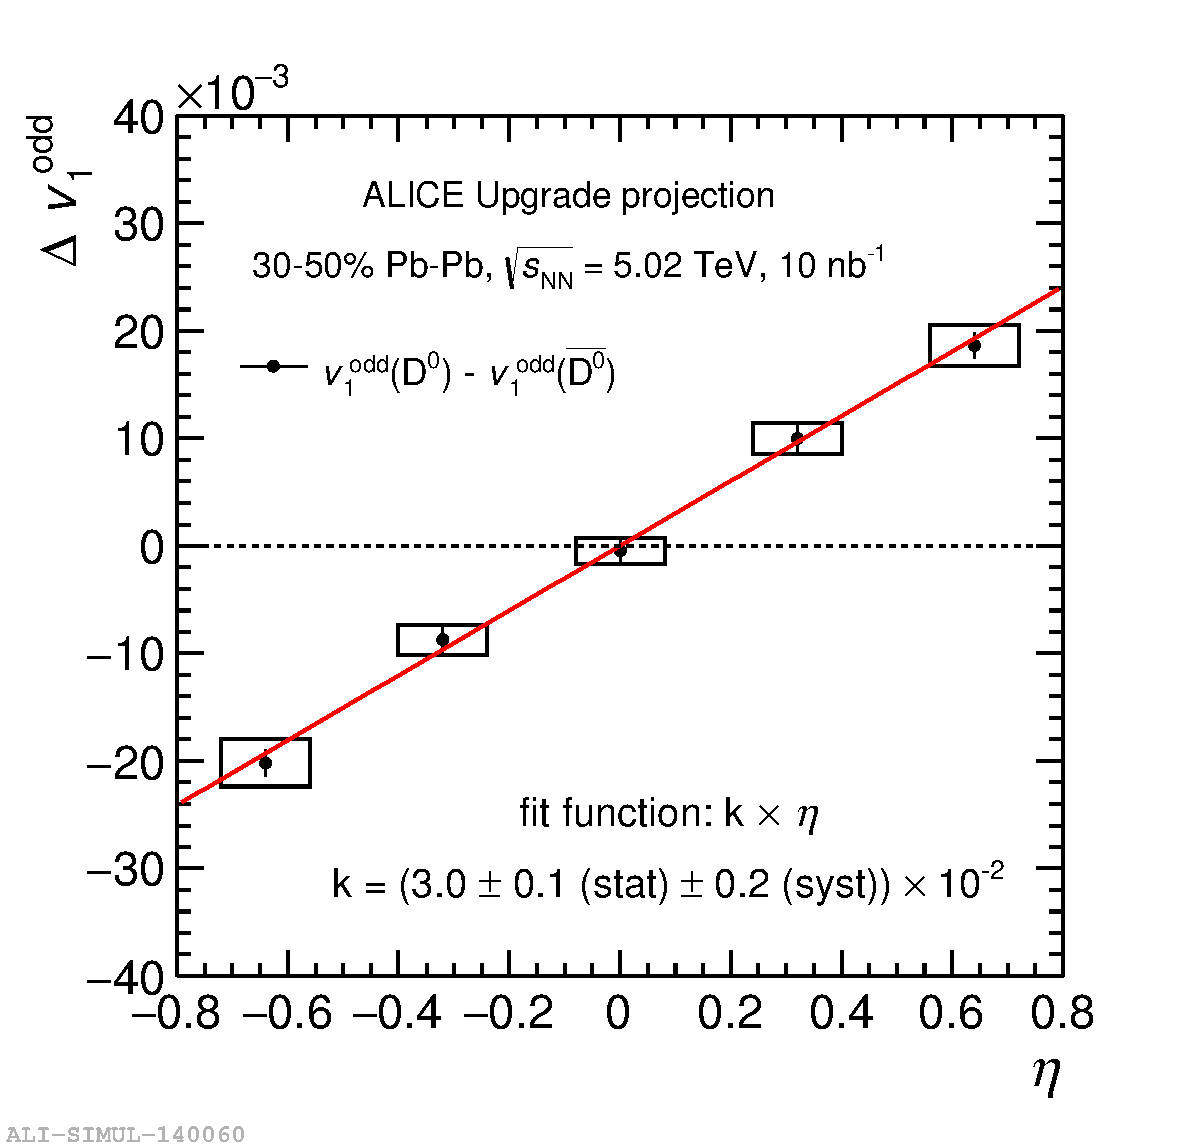
\includegraphics{hf/figures/2017-Oct-26-ALiceProjDeltav1Dzero.pdf}}
\caption{ALICE projection of the difference of directed flow $\vone$ for $\PDz$ and $\APDzero$ as a function of pseudorapidity in semi-central \PbPb collisions at $\sqrtsNN=$ 5.5 $\UTeV$.}
\label{fig:v1}
\end {figure}





% The presence of early magnetic fields produced in heavy-ion collisions is expected to have an effect on the charm directed flow~\cite{Das:2016cwd,Chatterjee:2018lsx,Plumari,Sandeep}, resulting in a $\vone$ value larger than that of lighter particles (short charm formation time and therefore sensitive to the maximum magnetic field strength), and opposite for particles with charm and anti-charm (due to the Lorentz force). Also the initial vorticity of non-central collision is expected to affect the directed flow observable.
% The STAR collaboration recently presented the first measurements of the directed flow $\vone$ coefficient for mesons~\cite{Singha}. This first observation of non-zero $\vone$ for charm mesons, and larger than that of lighter particles, is in qualitative agreement with theoretical models including both electromagnetic and vorticity effects. The uncertainties on the difference between the $\vone$ of $\PDz$ and $\APDzero$
% from STAR are still large to draw conclusions on the effects of the early magnetic fields.

% The LHC Run 3 and 4 will enable more precise measurements on the charm directed flow, which will give additional insights into the initial vorticity and electromagnetic fields, adding more constraints to the QGP properties. Figure~\ref{fig:v1} shows the precision level for the difference of directed flow $\vone$ for $\PDz$ and $\APDzero$ which ALICE can measure as a function of pseudorapidity in semi-central \PbPb collisions at $\sqrtsNN=$ 5.5 $\UTeV$.

% \begin{figure}
% \centering
% \resizebox{0.5\textwidth}{!}{  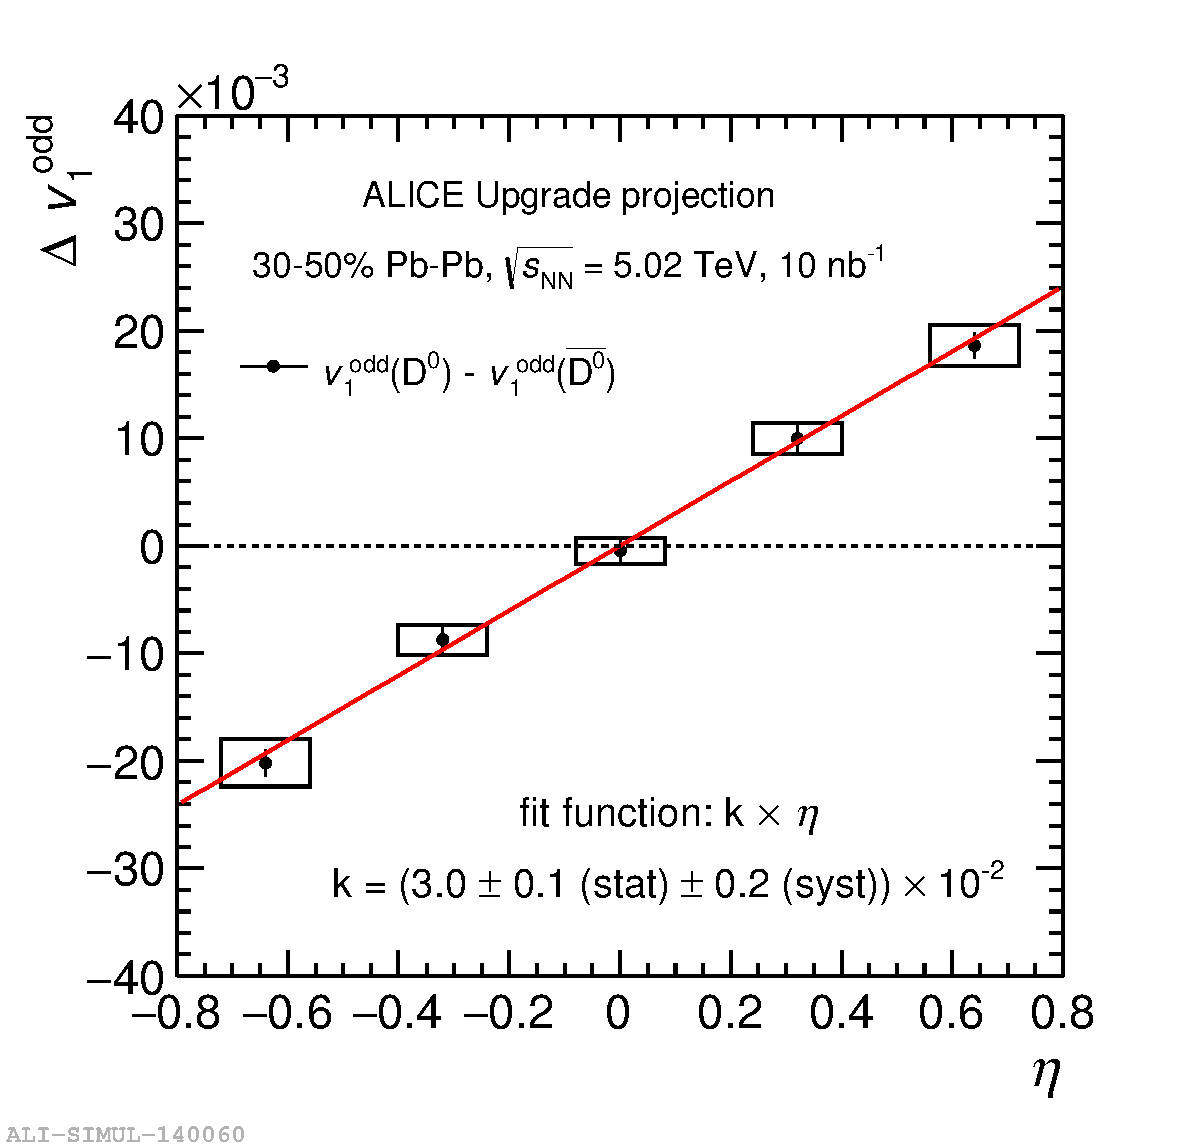
\includegraphics{hf/figures/2017-Oct-26-ALiceProjDeltav1Dzero.pdf}}
% \caption{ALICE projection of the difference of directed flow $\vone$ for $\PDz$ and $\APDzero$ as a function of pseudorapidity in semi-central Pb--Pb collisions at $\sqrtsNN=$ 5.5 $\UTeV$.}
% \label{fig:v1}
% \end {figure}

